\setcounter{figure}{14}
\begin{figure}[H]
\centering
\par\smallskip\textbf{Panel S15A analogue: different documented E1 event: partially reproduced}\par
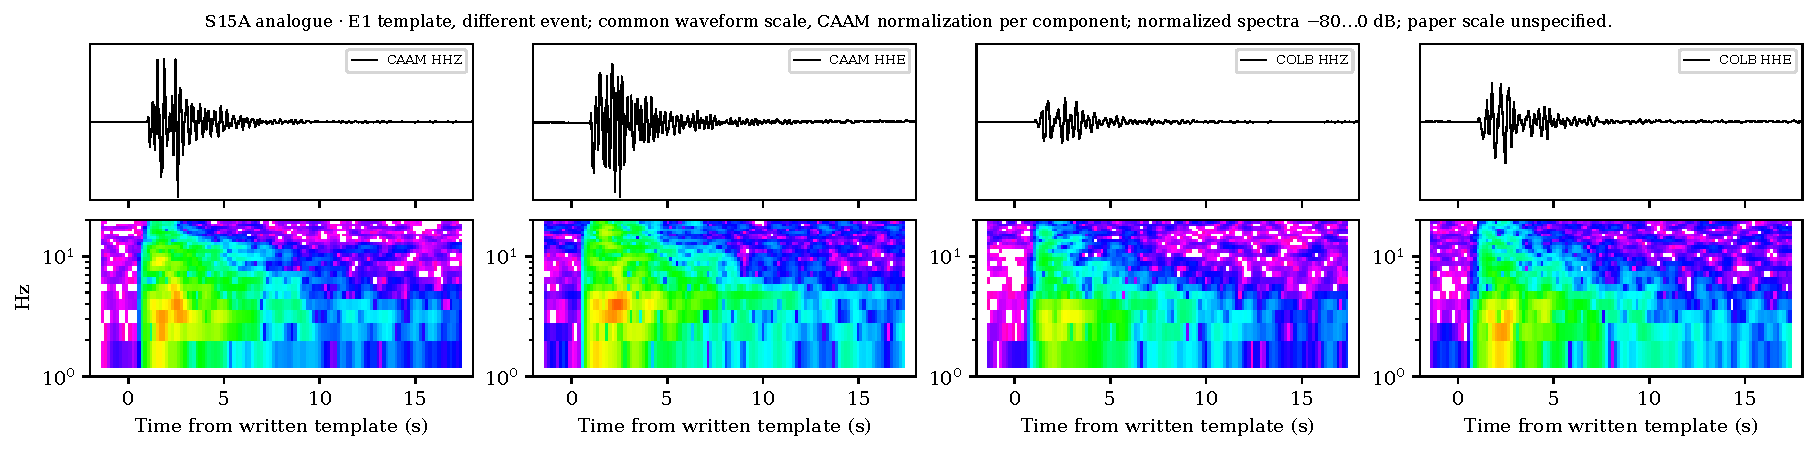
\includegraphics[width=.94\linewidth,height=0.207\textheight,keepaspectratio]{figures/hybrid_E1.pdf}
\par\smallskip\textbf{Panel S15B analogue: different documented E2 event: partially reproduced}\par
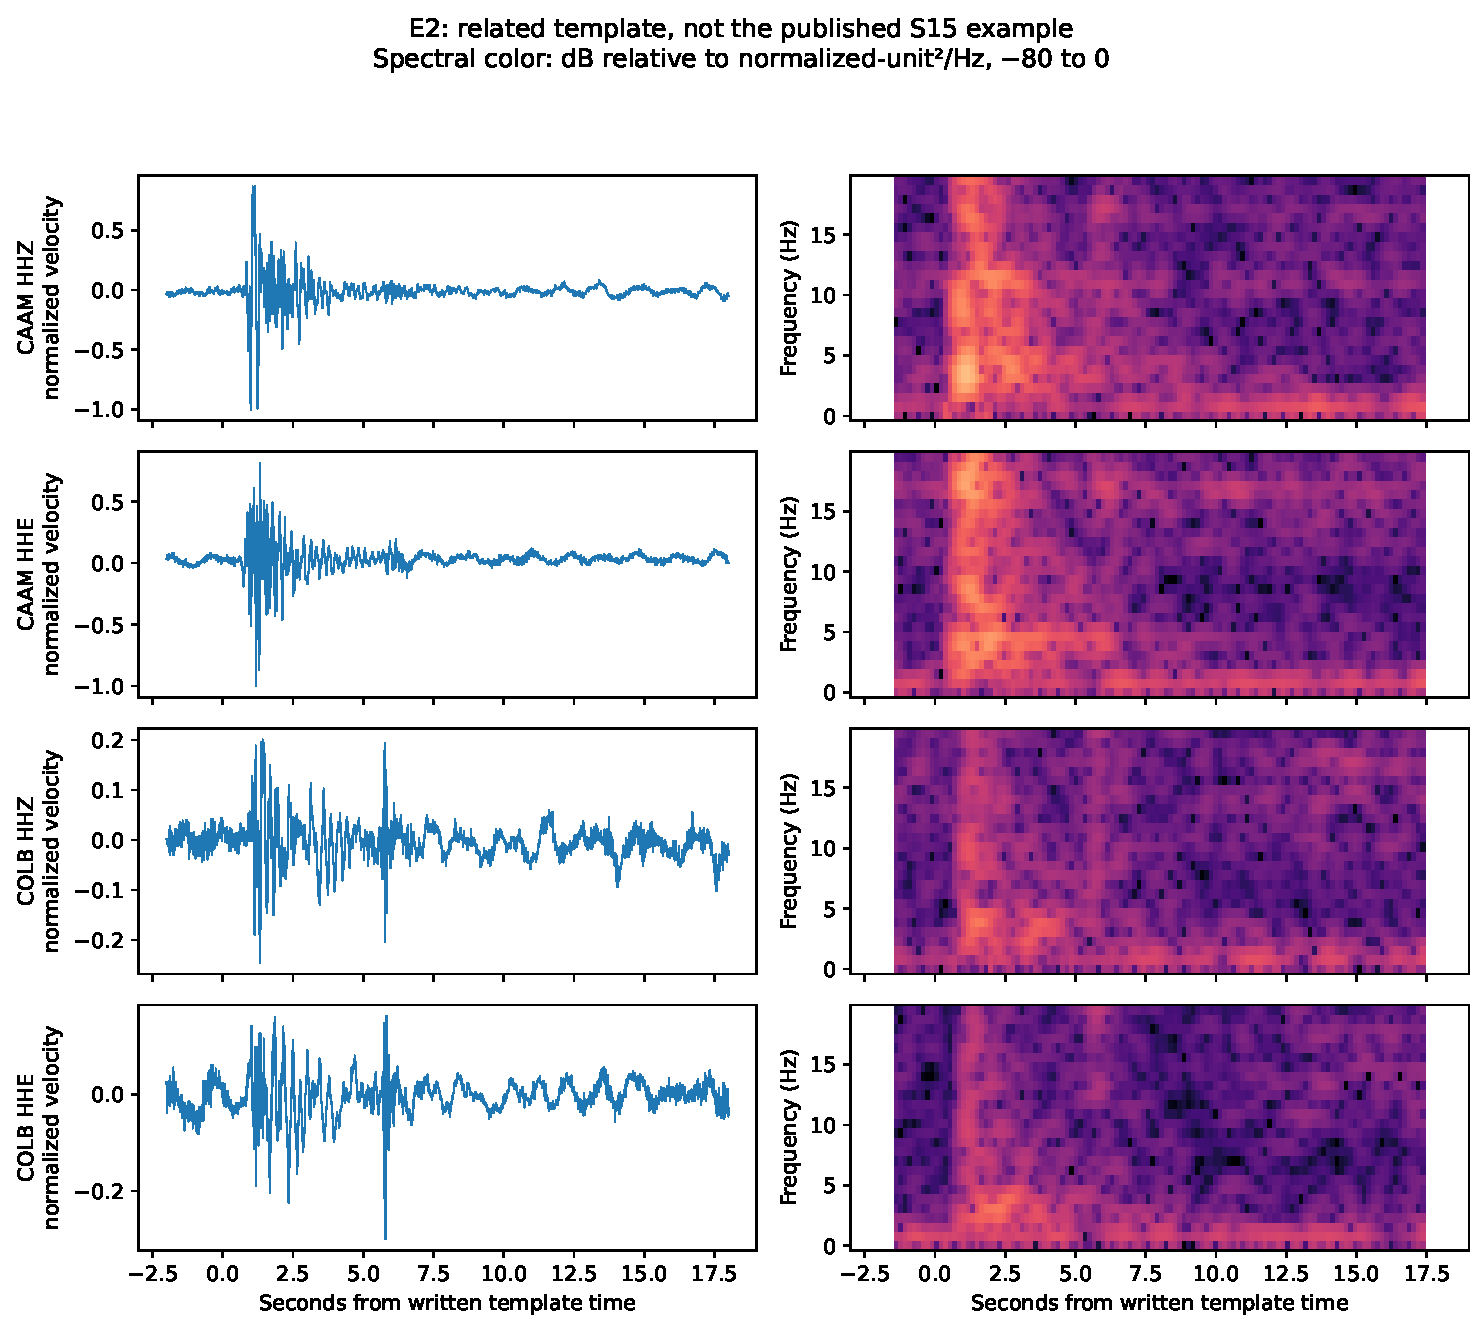
\includegraphics[width=.94\linewidth,height=0.207\textheight,keepaspectratio]{figures/hybrid_E2.pdf}
\par\smallskip\textbf{Panel S15C: documented E3 event: partially reproduced}\par
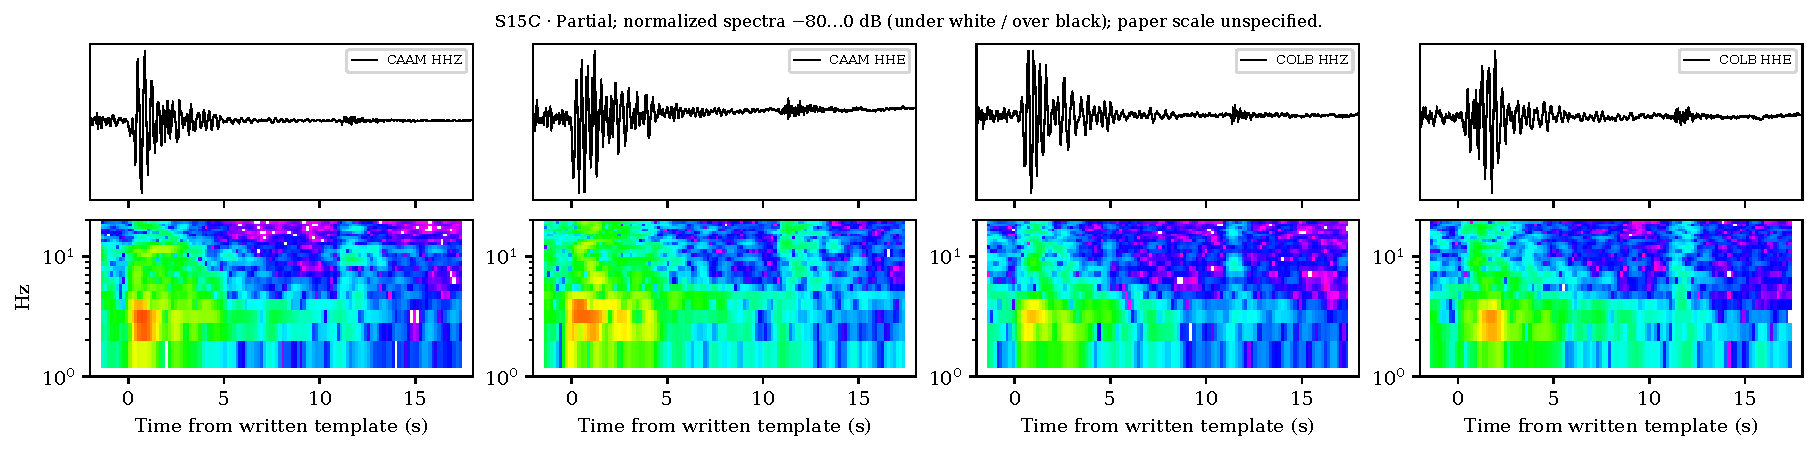
\includegraphics[width=.94\linewidth,height=0.207\textheight,keepaspectratio]{figures/hybrid_E3.pdf}
\par\small S15D: no retained independently relocated event with depth <0.6 km south of 40.83 N in this cohort, hence no suitable west-Accademia extremely-shallow example. Incorrectly labeled examples are not substituted.
\caption{Hybrid and shallow-event waveforms. Partial numerical waveform/spectral counterparts. A/B analogues use the written-method E1/E2 family templates, which are different events from the published A/B examples. They are explicitly not exact event reproduction. C uses E3. All are processed original CAAM/COLB observations; normalization and spectral settings are disclosed. No author waveform or spectral array is used.}
\label{publication:S15}
\end{figure}
